\documentclass{article}

%% Import any packages here
\usepackage{amsmath}
\usepackage{amsthm}
\usepackage{amssymb}
\usepackage[shortlabels]{enumitem}
\usepackage{graphicx}
\usepackage{xcolor}
\usepackage{fancyhdr}
\usepackage{hyperref}
\usepackage{physics}
\usepackage{tikz}


%% Define any custom commands/operators/environments/etc here
\newcommand{\Question}[1]{\Large \section{ #1 } \normalsize}

\DeclareMathOperator{\R}{\mathbb{R}}
\DeclareMathOperator*{\argmax}{arg\,max}
\DeclareMathOperator*{\argmin}{arg\,min}
\newcommand{\mat}[1]{\mathbf{#1}}
\renewcommand{\vec}[1]{\boldsymbol{\mathbf{#1}}}
\DeclareMathOperator*{\E}{\mathbb{E}}
\newcommand{\statind}{\perp\!\!\!\perp}

\newenvironment{solution}{\color{blue} \smallskip \textbf{Solution:}}{}

\paperwidth=8.5in
\paperheight=11in
\textheight=9in
\textwidth=7in
\hoffset=-0.25in
\voffset=-1in
\oddsidemargin=0in
\evensidemargin=0in
\parindent=0pt
\parskip=5pt
\itemsep=-1pt
\floatsep=9pt plus 2pt minus 3pt
\intextsep=9pt plus 2pt minus 3pt
\textfloatsep=9pt plus 2pt minus 3pt
\renewcommand{\baselinestretch}{1.1}

%% Page heading
\pagestyle{fancy}
\fancyhf{}
\setlength{\headheight}{30pt}
\lhead{\coursenumber, \semester}
\chead{\title}
\rhead{\name}
\lfoot{\class}
\rfoot{\thepage}

\def\coursenumber{CS 189/289A}
\def\class{Introduction to Machine Learning}
\def\semester{Fall 2024}
\def\name{Your Name} % Replace with your name
\def\title{HW 6}

\begin{document}
\fontsize{12}{15}\selectfont

\Question{Robot Localization with the Viterbi Algorithm}
Consider the following semi-realistic model of a robot's motion: we say that the state variable $X_t$ represents the robot's location in a grid-like environment. 
Suppose the grid has $r$ rows and $c$ columns. 
Then, there are $N = r \cdot c$ total states and the state space can be written as $\mathcal{S} = \{(i, j) \mid 0 \leq i < r,\; 0 \leq j < c\}$, i.e., each $X_t \in \mathcal{S}$ is represented by a tuple of row and column indices. 

This environment is enclosed by walls and has both horizontal and vertical walls scattered throughout between pairs of adjacent cells. 
Let $\mathrm{NEIGHBORS}(q)$ denote the set of empty grid cells that are adjacent to state $q$ and are reachable from it (i.e., not blocked from $q$ by a wall).
Then, we model the robot's motion in this environment as a random walk where it transitions to one of its unblocked neighboring cells uniformly at random, i.e.,
\[
    P(X_{t+1} = q' \mid X_t = q) = \frac{1}{|\mathrm{NEIGHBORS}(q)|} \;\text{ if }\; q' \in \mathrm{NEIGHBORS}(q) \;\text{ else }\; 0
\]
We don't know where the robot starts, so we will assume that the probability distribution $\pi$ over the initial states is uniform; that is $P(X_0 = (i, j)) = 1/N$.

The robot has 4 sensors mounted on it, one pointing in each of the 4 cardinal directions. 
Each sensor returns a single bit output: 1 when a sensor reads a wall directly in front of it and 0 if it reads open space. 
The observation at a timestep $t$ is a 4-bit sequence returning the sensor values from the left, right, up and down sensors respectively, \textbf{in that particular order}. 
For example, for the environment in the figure above, 
\begin{itemize}
    \item if the robot is present in the top left cell (i.e., $X_t = (0, 0)$), its sensors should read $1011$ because there is a wall in the left, up and down directions.
    \item if the robot is present in the top right cell (i.e., $X_t = (0, 15)$), its sensors should read $0110$ because there are walls in the right and up directions.
\end{itemize} 
We note that the number of 0s that a sensor should read in state $q$ is precisely $|\mathrm{NEIGHBORS}(q)|$.

However, the sensors are faulty! 
Each sensor, independent of the others and the timestep, can fail with probability $\epsilon$ and incorrectly flip its output. 
Therefore, there are $2^4$ possible observations that we can read off of the robot, each occurring with different probabilities: if there are $d$ discrepancies between the true sensor reading and the returned sensor reading, the probability of this observation will be $(1 - \epsilon)^{4 - d}\epsilon^d$.

The true robot states $X_t$ are hidden from us, but we can observe the faulty sensor readings, say denoted by $Y_t$ at timestep $t$, every time the robot moves to a new state. 
As such, we can model the scenario above using a hidden markov model.

\begin{enumerate}[(a)]
    \item 
    Our goal is to predict the true robot hidden states from the observed sensor readings. 
    Given a sequence of $T$ observations $o_1, \dots, o_T$, \textbf{implement the Viterbi algorithm to decode the most likely sequence of hidden states.} 
    You have all the information required to compute the transition probabilities $P(X_{t+1} = q' \mid X_t = q)$ and observation emission probabilities $P(Y_t = o_t \mid X_t = q)$.

    The starter code contains two files:
    \begin{itemize}
        \item \texttt{env.py}: This file encodes the dynamics of the environment.
        In particular, it defines the \texttt{Env} class which creates the underlying environment, tracks the true robot hidden state and emits sensor readings.  
        % Feel free to read through this file, but you don't need to understand the code here to work on this problem. 
        You may call any pre-defined methods of the \texttt{Env} class but not access any of its instance variables from \texttt{hmm.py}.
        \item \texttt{hmm.py}: This is where all of your code should go.
    \end{itemize}

    Since your goal is to return the best set of hidden states, \textbf{don't forget to also backtrace your way through the viterbi probabilities} to find the most likely sequence. Feel free to reference \href{https://web.stanford.edu/~jurafsky/slp3/A.pdf}{\textbf{this handout on HMMs}} for more information about the Viterbi algorithm.

    \textbf{Include your code in the appendix and select the appropriate pages when submitting to Gradescope. Also submit \texttt{hmm.py} to the Gradescope coding assignment.}

    \item 
    Now, we will vary the error parameter $\epsilon$ to values like $0$, $0.05$, $0.1$, $0.2$, $0.25$ and $0.5$. For each value of epsilon, we will generate and decode 100 sequences of 100 observations each. We also plot the cumulative accuracy (i.e., the accuracy of the first $i$ predictions when compared to the first $i$ hidden states, for each $i \in [1, 100]$, for a single trajectory), averaged over all 100 trajectories, for each $\epsilon$. Attach this plot in your writeup. Describe any trends that you see in the plot: what happens when $\epsilon$ increases from 0 to 0.5? for a fixed epsilon, how does the cumulative accuracy change over time? Do these trends align with your intuition?

    \begin{solution}
        TODO
    \end{solution}
\end{enumerate}


\newpage
\Question{Graphical Model Potpourri}
\begin{enumerate}[(a)]
    \item
    Show that $a \statind (b, c) \mid d$ implies $a \statind b \mid d$.

    \begin{solution}
        TODO
    \end{solution}

    \newpage
    \item 
    Suppose you have a set of $d$ binary random variables $\{X_1, ..., X_d\}$.
    \begin{enumerate}[(i)]
        \item 
        Without making any independence assumptions, what is the minimum number of parameters needed to fully specify the joint distribution? \\
        \textit{Hint:} You need one fewer parameter compared to the number of outcomes, due to the constraint that the total probability should sum to $1$.

        \begin{solution}
            TODO
        \end{solution}
        
        \item 
        Suppose the random variables are structured as a Markov chain, where each $X_i$ only depends on $X_{i-1}$. What is the minimum number of parameters needed now?

        \begin{solution}
            TODO
        \end{solution}
        
        \item 
        How does the parameter complexity change going from no independence assumption to a Markovian assumption?

        \begin{solution}
            TODO
        \end{solution}
    \end{enumerate}

    \newpage
    \item 
    Consider the following three graphical models with distinct structures.
    \begin{center}
        \begin{tikzpicture}
            % G1 structure
            \node[circle, draw=black, minimum size=1cm] (a1) at (0, -1.5) {$a$};
            \node[circle, draw=black, minimum size=1cm] (c1) at (1.75, -1.5) {$c$};
            \node[circle, draw=black, minimum size=1cm] (b1) at (3.5, -1.5) {$b$};
            \draw[->, black] (a1) -- (c1);
            \draw[->, black] (c1) -- (b1);
            \node at (1.75, -4) {G1};
        
            % Vertical bar between G1 and G2
            \draw[thick] (4.5, -0.5) -- (4.5, -4.5);
        
            % G2 Common Cause structure
            \node[circle, draw=black, minimum size=1cm] (c2) at (7, -1.5) {$c$};
            \node[circle, draw=black, minimum size=1cm] (a2) at (5.5, -3) {$a$};
            \node[circle, draw=black, minimum size=1cm] (b2) at (8.5, -3) {$b$};
            \draw[->, black] (c2) -- (a2);
            \draw[->, black] (c2) -- (b2);
            \node at (7, -4) {G2};
        
            % Vertical bar between G2 and G3
            \draw[thick] (9.5, -0.5) -- (9.5, -4.5);
        
            % G3 Common Effect structure
            \node[circle, draw=black, minimum size=1cm] (c3) at (12, -3) {$c$};
            \node[circle, draw=black, minimum size=1cm] (a3) at (10.5, -1.5) {$a$};
            \node[circle, draw=black, minimum size=1cm] (b3) at (13.5, -1.5) {$b$};
            \draw[->, black] (a3) -- (c3);
            \draw[->, black] (b3) -- (c3);
            \node at (12, -4) {G3};
        \end{tikzpicture}
    \end{center}
    Match each scenario to the most appropriate graphical model.
    \begin{enumerate}[(i)]
        \item 
        A family’s decision on where to travel (\(c\)) involves considerations such as the parents' work schedules (\(a\)) and the children’s school holidays (\(b\)).

        \begin{solution}
            TODO
        \end{solution}
        
        \item 
        A record-breaking snowfall (\(c\)) spurs both ski resort bookings (\(a\)) and demand for winter clothing (\(b\)).

        \begin{solution}
            TODO
        \end{solution}

        \item 
        A person's workout routine (\(a\)) affects their energy levels (\(c\)), which then influences their work productivity (\(b\)).

        \begin{solution}
            TODO
        \end{solution}

        \item 
        The climate of a region (\(a\)) impacts the type of vegetation that grows (\(c\)), which in turn determines the wildlife population (\(b\)).

        \begin{solution}
            TODO
        \end{solution}

        \item 
        A country's economic stability (\(c\)) affects both employment rates (\(a\)) and consumer spending habits (\(b\)).

        \begin{solution}
            TODO
        \end{solution}

        \item 
        A restaurant’s popularity (\(c\)) hinges on both the quality of its food (\(a\)) and its social media presence (\(b\)).

        \begin{solution}
            TODO
        \end{solution}
    \end{enumerate}

    \newpage
    \item 
    Consider the following directed graph, where none of the variables are observed. 

    \begin{figure}[h]
        \centering
        \begin{tikzpicture}
            \node[circle, draw=black, thick, minimum size=1cm] (a) at (-1.5, 2) {\(a\)};
            \node[circle, draw=black, thick, minimum size=1cm] (b) at (3.5, 2) {\(b\)};
            \node[circle, draw=black, thick, minimum size=1cm] (c) at (1, 1) {\(c\)};
            \node[circle, draw=black, thick, minimum size=1cm] (d) at (1, -1.5) {\(d\)};
            \draw[->, thick, black] (a) -- (c);
            \draw[->, thick, black] (b) -- (c);
            \draw[->, thick, black] (c) -- (d);
        \end{tikzpicture}
    \end{figure}

    \begin{enumerate}[(i)]
        \item 
        What is the joint distribution $p(a, b, c, d)$ in terms of the marginal and conditional distributions given in the graph?

        \begin{solution}
            TODO
        \end{solution}

        \item 
        Assuming that $a, b, c, d$ are binary random variables, what is the minimum number of parameters required to specify the joint distribution?

        \begin{solution}
            TODO
        \end{solution}

        \item 
        Show that $a$ and $b$ are independent, or \(a \statind b\). 

        \begin{solution}
            TODO
        \end{solution}

        \item 
        Assume that for any given node $x$ in the graph, $p(x \mid \text{pa}(x)) \neq p(x)$, where $\text{pa}(\cdot)$ denotes the parent nodes of $x$. 
        Show that when $d$ is observed, $a$ and $b$ are no longer independent, or \(a \not\statind b \mid d\). 

        \begin{solution}
            TODO
        \end{solution}
    \end{enumerate}
\end{enumerate}


\newpage
\Question{Langevin Dynamics Demo}
\newcommand{\notebookurl}{https://colab.research.google.com/drive/1fvcWjRJYRLQM83RPKu-uQ4sqAPGTuuxA?usp=sharing} 

For this question, go to the Google Colab notebook provided \href{\notebookurl}{\textbf{\emph{here}}} \footnote{\href{\notebookurl}{\notebookurl}} to complete the code.

In this notebook, we will walk through a simple demo for Langevin dynamics, where the goal is to sample from a distribution $\text{p}(x)$ using only its score function $\nabla_x \text{log} \text{p}(x)$. 
Here we assume a toy setting where $\text{p}(x)$ is known. 
In most practical cases we only have access a dataset of samples $\mathcal{D} = \{x_0, x_1, \ldots, x_n\} \sim p(x)$, in which case we might use a technique called score matching to estimate the score function\footnote{\href{https://papers.neurips.cc/paper\_files/paper/2019/hash/3001ef257407d5a371a96dcd947c7d93-Abstract.html}{Yang Song and Stefano Ermon. Generative modeling by estimating gradients of the data distribution. NeurIPS 2019.}}. 
For more background, you can reference Chapter 14.3 on Langevin Sampling in \href{https://www.bishopbook.com}{Bishop and Bishop, 2024}.

Recall that the Langevin update equation at timestep $t$ with step size $\eta$ and random noise $\epsilon \sim \mathcal{N}(0,I)$ is
\[
    x_{t+1} = x_t + \eta\nabla_x \log p(x) + \sqrt{2\eta}\epsilon
\]
\textbf{Deliverables:} Complete the written questions below, which will walk you through the notebook. In addition, submit the .ipynb file to the code assignment.

\begin{enumerate}
    \item 
    Complete the functions \texttt{langevin\_update} and \texttt{sample\_langevin}. Include a PDF export of the completed code in your write-up.

    \begin{solution}
        TODO
    \end{solution}

    \item
    Using the given default settings, visualize the samples over time. 
    Include an image of the plots and describe what you see. 
    Which is closer to the target shape, early or late timesteps? 
    How does the variance of the samples change over time? \\
    \textit{Note:} To simplify the runtime and plotting, throughout this problem you will only run the Langevin sampler for a few iterations. 
    In practice, however, you would typically run the sampler for longer (e.g., several thousand iterations), to ensure the Markov chain has converged.

    \begin{solution}
        TODO
    \end{solution}

    \item 
    Now let's adjust the radius of the elliptical logpdf. 
    Set \texttt{rx, ry = 1.0, 2.5}. 
    How do the final samples compare with the samples for the circular logpdf? 
    Does Langevin sampling fit better to the elliptical or the circular logpdf? \\
    \textit{Hint:} Even coverage over the entire target distribution is more desirable.

    \begin{solution}
        TODO
    \end{solution}

    \item 
    Let's see if we can get a better fit to the elliptical logpdf in (c) by tuning each dimension of \texttt{eta}. 
    What is a better selection of \texttt{eta}?

    \begin{solution}
        TODO
    \end{solution}

    \item 
    Here let's move the center of the logpdf away from the origin. 
    Set \texttt{rx, ry = 1.5, 1.5} and \texttt{cx, cy = 1.0, 1.0}. 
    How do the final samples compare with centered logpdf? 
    Does Langevin sampling fit better to the centered or off-center logpdf?

    \begin{solution}
        TODO
    \end{solution}

    \item 
    For the off-centered logpdf in (e), let's try to get a better fit by tuning the initialization
    \texttt{init\_particles}. What can you do to improve the initialization?

    \begin{solution}
        TODO
    \end{solution}
\end{enumerate}

\end{document}